\begin{titlepage}
    \begin{center}
    	%\thispagestyle{firstpage} % Apply the page style for the first page (no headers and footers)
    	\pagenumbering{gobble}
        %\vspace*{1cm}
        \usefont{OT1}{phv}{m}{it} %change font for date only
        \maketitle % Print the title
        \normalfont %reset to default font
        
        
        \lettrineabstract{The specificity of DNA base-pair interactions gives considerable functional control in the design of anisotropic nano-particles, enabling the formation of a range of liquid crystal phases. Initial benchmarked tests, performed using a course-grained model that reflects the DNA-mesogens used in experiments, confirm the critical volume fraction of the nematic phase transition for linear double-stranded (ds) DNA mesogens to within 5\% of the theoretical value over a range of aspect ratios. I then introduce a novel `nunchuck' mesogen -- two rigid rods of ds-DNA connected via a flexible linker of single-stranded (ss) DNA, and demonstrate the existence of an entropy-driven phase transition to a quasi-nematic (S = 0.58) phase in this system. I outline further evidence for the existence of more exotic `herringbone', twisted-nematic and biaxial-nematic phases through the use of the pair-wise orientational correlation function. Finally, I present an alternative method for phase identification through the study of dynamic properties, and identify the formation of nematic and smectic phases through the measurement of directional diffusion coefficients of the mesogens.}
        
%        \begin{figure}[h!]
%        	\centering
%        	
\includegraphics[width=0.4\linewidth]{Figures/university-of-cambridge-seeklogo.com}
%        	\caption*{}
%        \end{figure}

      
\vspace*{1.2cm}

        \begin{figure}[h!]
        	\centering
        	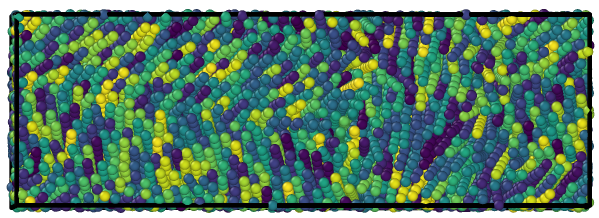
\includegraphics[width=0.9\linewidth]{Figures/nun_fa_twist}
        	\caption*{An exotic twisted-nematic structure formed by a system of 1000 nunchucks.}
        \end{figure}  
        
%        Supplementary Material: \textit{If necessary} \\
%		Online Lab-book: \textit{To be included} \\
		
\vspace*{1.2cm}

Except where specific reference is made to the work of others,\\ this work is original and has not been already submitted, either wholly or in part,\\ to satisfy any degree requirement at this or any other university.
        
       
        
    \end{center}
\end{titlepage}